%% abtex2-modelo-trabalho-academico.tex, v-1.8 laurocesar
%% Copyright 2012-2013 by abnTeX2 group at http://abntex2.googlecode.com/ 
%%
%% This work may be distributed and/or modified under the
%% conditions of the LaTeX Project Public License, either version 1.3
%% of this license or (at your option) any later version.
%% The latest version of this license is in
%%   http://www.latex-project.org/lppl.txt
%% and version 1.3 or later is part of all distributions of LaTeX
%% version 2005/12/01 or later.
%%
%% This work has the LPPL maintenance status `maintained'.
%% 
%% The Current Maintainer of this work is the abnTeX2 team, led
%% by Lauro César Araujo. Further information are available on 
%% http://abntex2.googlecode.com/
%%
%% This work consists of the files abntex2-modelo-trabalho-academico.tex,
%% abntex2-modelo-include-comandos and abntex2-modelo-references.bib
%%

% ------------------------------------------------------------------------
% ------------------------------------------------------------------------
% abnTeX2: Modelo de Trabalho Academico (tese de doutorado, dissertacao de
% mestrado e trabalhos monograficos em geral) em conformidade com 
% ABNT NBR 14724:2011: Informacao e documentacao - Trabalhos academicos -
% Apresentacao
% ------------------------------------------------------------------------
% ------------------------------------------------------------------------

\documentclass[
	% -- opções da classe memoir --
	12pt,				% tamanho da fonte
	%openright,			% capítulos começam em pág ímpar (insere página vazia caso preciso)
	%twoside,			% para impressão em verso e anverso. Oposto a oneside
	oneside,			% para impressão em verso e anverso. Oposto a oneside
	a4paper,			% tamanho do papel. 
	% -- opções da classe abntex2 --
	%chapter=TITLE,		% títulos de capítulos convertidos em letras maiúsculas
	%section=TITLE,		% títulos de seções convertidos em letras maiúsculas
	%subsection=TITLE,	% títulos de subseções convertidos em letras maiúsculas
	%subsubsection=TITLE,% títulos de subsubseções convertidos em letras maiúsculas
	% -- opções do pacote babel --
	english,			% idioma adicional para hifenização
	brazil,				% o último idioma é o principal do documento
	]{ime-abntex2}


% ---
% PACOTES
% ---

% ---
% Pacotes fundamentais 
% ---
\usepackage[utf8]{inputenc}		% Codificacao do documento (conversão automática dos acentos)
\usepackage{cmap}			% Mapear caracteres especiais no PDF
%\usepackage{lmodern}			% Usa a fonte Latin Modern
\usepackage{amsmath}			% Para usar fontes ams
\usepackage{amsfonts}			% Para usar fontes ams
\usepackage[T1]{fontenc}		% Selecao de codigos de fonte.
%\usepackage{lastpage}			% Usado pela Ficha catalográfica
\usepackage{indentfirst}		% Indenta o primeiro parágrafo de cada seção.
\usepackage{color}			% Controle das cores
\usepackage{graphicx}			% Inclusão de gráficos
\usepackage{algorithm2e}		% Para escrever algorítimos
% o seguinte é necessário para corrigir um bug no algorithm2e
% http://tex.stackexchange.com/questions/113325/problem-with-algorithm2e-and-portuguese-option
\SetKwFor{Para}{para}{fa\c{c}a}{fim para}
% não era pra precisar do seguinte, mas precisa para traduzir a captions dos algoritmos
\renewcommand{\algorithmcfname}{Algoritmo}%
% ---

% ---
% Pacotes adicionais, usados apenas no âmbito do documento em questão
% ---
%\usepackage{lipsum}			% para geração de dummy text
% ---

% ---
% Pacotes de citações
% ---
\usepackage[brazilian,hyperpageref]{backref}	 % Paginas com as citações na bibl
\usepackage[alf]{abntex2cite}	% Citações padrão ABNT

% --- 
% CONFIGURAÇÕES DE PACOTES
% --- 

% ---
% Configurações do pacote backref
% Usado sem a opção hyperpageref de backref
\renewcommand{\backrefpagesname}{Citado na(s) página(s):~}
% Texto padrão antes do número das páginas
\renewcommand{\backref}{}
% Define os textos da citação
\renewcommand*{\backrefalt}[4]{
	\ifcase #1 %
		Nenhuma citação no texto.%
	\or
		Citado na página #2.%
	\else
		Citado #1 vezes nas páginas #2.%
	\fi}%
% ---


% ---
% Informações de dados para CAPA e FOLHA DE ROSTO
% ---
\titulo{Heurística Estática para Times\\Cooperativos de Robôs}
\autor{
  Jan Segre\\
  Victor Bramigk
}
\local{Rio de Janeiro}
\data{Outubro de 2013}
\orientador{Paulo F. F. Rosa - Ph.D}
%\coorientador{Equipe \abnTeX}
\instituicao{%
  Instituto Militar de Engenharia
  \par
  Seção de Computação
  \par
  Graduação em Engenharia de Computação}
\tipotrabalho{Iniciação à Pesquisa}
% O preambulo deve conter o tipo do trabalho, o objetivo, 
% o nome da instituição e a área de concentração 
\preambulo{Iniciação à Pesquisa apresentada ao Curso de Graduação
em Engenharia de Computação do Instituto Militar de
Engenharia.}
% ---


% ---
% Configurações de aparência do PDF final

% alterando o aspecto da cor azul
%\definecolor{blue}{RGB}{41,5,195}
\definecolor{blue}{RGB}{0,0,0}

% informações do PDF
\makeatletter
\hypersetup{
	%pagebackref=true,
	pdftitle={\@title},
	pdfauthor={\@author},
	pdfsubject={\imprimirpreambulo},
	pdfcreator={LaTeX with abnTeX2},
	pdfkeywords={ime}{robocup}{analise}{logs}{rede neural},
	colorlinks=true,		% false: boxed links; true: colored links
	linkcolor=blue,			% color of internal links
	citecolor=blue,			% color of links to bibliography
	filecolor=magenta,		% color of file links
	urlcolor=blue,
	bookmarksdepth=4
}
\makeatother
% ---

% ---
% Espaçamentos entre linhas e parágrafos 
% ---

% O tamanho do parágrafo é dado por:
%\setlength{\parindent}{1.3cm}

% Controle do espaçamento entre um parágrafo e outro:
%\setlength{\parskip}{0.2cm}  % tente também \onelineskip
\setlength{\parskip}{\onelineskip}

% ---
% compila o indice
% ---
\makeindex
% ---

% ----
% Início do documento
% ----
\begin{document}

% Retira espaço extra obsoleto entre as frases.
%\frenchspacing

% ----------------------------------------------------------
% ELEMENTOS PRÉ-TEXTUAIS
% ----------------------------------------------------------
% \pretextual

% ---
% Capa
% ---
\imprimircapa
%\begin{center}
\textbf{MINISTÉRIO DA DEFESA}\\
\textbf{EXÉRCITO BRASILEIRO}\\
\textbf{DEPARTAMENTO DE CIÊNCIA E TECNOLOGIA}\\
\textbf{INSTITUTO MILITAR DE ENGENHARIA}\\
\textbf{Seção de Engenharia de Sistemas / SE 8}

\vspace{2.5cm}

\begin{large}
\textbf{Proposta de Tema de Dissertação de Mestrado
\\Curso: Mestrado em Sistemas e Computação}

\vspace{1.5cm}

\textbf{Sistema de Localização de Objetos para Apoio a um Assistente Robótico Móvel na Casa Inteligente}

\vspace{1.5cm}

\textbf{Aluno: Fulano}

\vspace{1.5cm}

\textbf{Orientador: Paulo F. F. Rosa, Ph.D}

\end{large}

\vspace{2cm}

\begin{small}
Data de Apresentação no SE/8:\\
Rio de Janeiro, \today
\end{small}

\end{center}

\pagebreak

% ---

% ---
% Folha de rosto
% (o * indica que haverá a ficha bibliográfica)
% ---
\imprimirfolhaderosto*
%\maketitle

% ---

% ---
% Inserir a ficha bibliografica
% ---

% Isto é um exemplo de Ficha Catalográfica, ou ``Dados internacionais de
% catalogação-na-publicação''. Você pode utilizar este modelo como referência. 
% Porém, provavelmente a biblioteca da sua universidade lhe fornecerá um PDF
% com a ficha catalográfica definitiva após a defesa do trabalho. Quando estiver
% com o documento, salve-o como PDF no diretório do seu projeto e substitua todo
% o conteúdo de implementação deste arquivo pelo comando abaixo:
%
% \begin{fichacatalografica}
%     \includepdf{fig_ficha_catalografica.pdf}
% \end{fichacatalografica}
\imprimirfichacatalografica
{xxxx}
{Segre, J., Bramigk, V.}
{1. Engenharia da computação.
 2. Redes Neurais.
 3. Lógica Nebulosa.
 4. Otimização da Colônia de Formigas. Instituto Militar de Engenharia.}
% ---

% ---
% Inserir errata
% ---
%\begin{errata}
%Elemento opcional da \citeonline[4.2.1.2]{NBR14724:2011}. Exemplo:
%
%\vspace{\onelineskip}
%
%FERRIGNO, C. R. A. \textbf{Tratamento de neoplasias ósseas apendiculares com
%reimplantação de enxerto ósseo autólogo autoclavado associado ao plasma
%rico em plaquetas}: estudo crítico na cirurgia de preservação de membro em
%cães. 2011. 128 f. Tese (Livre-Docência) - Faculdade de Medicina Veterinária e
%Zootecnia, Universidade de São Paulo, São Paulo, 2011.
%
%\begin{table}[htb]
%\center
%\footnotesize
%\begin{tabular}{|p{1.4cm}|p{1cm}|p{3cm}|p{3cm}|}
%  \hline
%   \textbf{Folha} & \textbf{Linha}  & \textbf{Onde se lê}  & \textbf{Leia-se}  \\
%    \hline
%    1 & 10 & auto-conclavo & autoconclavo\\
%   \hline
%\end{tabular}
%\end{table}
%
%\end{errata}
% ---

% ---
% Inserir folha de aprovação
% ---
%
% Isto é um exemplo de Folha de aprovação, elemento obrigatório da NBR
% 14724/2011 (seção 4.2.1.3). Você pode utilizar este modelo até a aprovação
% do trabalho. Após isso, substitua todo o conteúdo deste arquivo por uma
% imagem da página assinada pela banca com o comando abaixo:
%
% \includepdf{folhadeaprovacao_final.pdf}
%
\convidadoum{Maj Julio Cesar Duarte - D.Sc. do IME}{}
\convidadodois{Ricardo Choren Noya - Ph.D do IME}{}
\imprimirfolhadeaprovacao{9 de outubro de 2013}
% ---

% ---
% Dedicatória
% ---
%\begin{dedicatoria}
%   \vspace*{\fill}
%   \centering
%   \noindent
%   \textit{ Este trabalho é dedicado às crianças adultas que,\\
%   quando pequenas, sonharam em se tornar cientistas.} \vspace*{\fill}
%\end{dedicatoria}
% ---

% ---
% Agradecimentos
% ---
%\begin{agradecimentos}
%Os agradecimentos principais são direcionados à Gerald Weber, Miguel Frasson,
%Leslie H. Watter, Bruno Parente Lima, Flávio de Vasconcellos Corrêa, Otavio Real
%Salvador, Renato Machnievscz\footnote{Os nomes dos integrantes do primeiro
%projeto abn\TeX\ foram extraídos de
%\url{http://codigolivre.org.br/projects/abntex/}} e todos aqueles que
%contribuíram para que a produção de trabalhos acadêmicos conforme
%as normas ABNT com \LaTeX\ fosse possível.
%
%Agradecimentos especiais são direcionados ao Centro de Pesquisa em Arquitetura
%da Informação\footnote{\url{http://www.cpai.unb.br/}} da Universidade de
%Brasília (CPAI), ao grupo de usuários
%\emph{latex-br}\footnote{\url{http://groups.google.com/group/latex-br}} e aos
%novos voluntários do grupo
%\emph{\abnTeX}\footnote{\url{http://groups.google.com/group/abntex2} e
%\url{http://abntex2.googlecode.com/}}~que contribuíram e que ainda
%contribuirão para a evolução do \abnTeX.
%
%\end{agradecimentos}
% ---

% ---
% Epígrafe
% ---
%\begin{epigrafe}
%    \vspace*{\fill}
%	\begin{flushright}
%		\textit{``Não vos amoldeis às estruturas deste mundo, \\
%		mas transformai-vos pela renovação da mente, \\
%		a fim de distinguir qual é a vontade de Deus: \\
%		o que é bom, o que Lhe é agradável, o que é perfeito.\\
%		(Bíblia Sagrada, Romanos 12, 2)}
%	\end{flushright}
%\end{epigrafe}
% ---

% ---
% RESUMOS
% ---

% resumo em português
\setlength{\absparsep}{18pt} % ajusta o espaçamento dos parágrafos do resumo
\begin{resumo}

O objetivo deste trabalho é prever como um time de futebol de robôs irá se comportar baseado
somente nas posições e orientações de um conjunto discreto de amostras. Para isso, foram estudados
os métodos da ACO (Ant Colony Optimization), SA (Simulated Annealing), Algorítimo  Genético, Lógica Nebulosa
e Redes Neurais. A partir do estudo detalhado desse algoritmos definiu-se duas linhas principais de
ação para a solução do problema: uma baseada em Logica Nebulosa e a outra baseada em Redes Neurais. Após
um estudo mais aprofundado deseja-se implementar um processo de otimização em ambos os algorítimos para
que o resultado seja refinado.

% Segundo a \citeonline[3.1-3.2]{NBR6028:2003}, o resumo deve ressaltar o
% objetivo, o método, os resultados e as conclusões do documento. A ordem e a extensão
% destes itens dependem do tipo de resumo (informativo ou indicativo) e do
% tratamento que cada item recebe no documento original. O resumo deve ser
% precedido da referência do documento, com exceção do resumo inserido no
% próprio documento. (\ldots) As palavras-chave devem figurar logo abaixo do
% resumo, antecedidas da expressão Palavras-chave:, separadas entre si por
% ponto e finalizadas também por ponto.
%
% \textbf{Palavras-chaves}: latex. abntex. editoração de texto.
\end{resumo}

% resumo em inglês
\begin{resumo}[Abstract]
\begin{otherlanguage*}{english}

The main objective of this work is predicting how a robot soccer team whill behave, based
on a set of positions and orientations of a discrete sample. For that, some heuristics were
studied: ACO (Ant Colony Optimization), SA (Simulated Annealing), GA (Genetic Algorithm),
and Neural Networks. Based on the detailed study of these algorithms two branches were defined
as candidate solutions: one based on the Neural Network heuristics, and the other based on
Fuzzy logic. After a deeper study on of these methods it's desirable to implement an algori-
thm which will refinethe result.

%\vspace{\onelineskip}

%\noindent
%\textbf{Key-words}: latex. abntex. text editoration.
\end{otherlanguage*}
\end{resumo}

% resumo em francês 
%\begin{resumo}[Résumé]
% \begin{otherlanguage*}{french}
%    Il s'agit d'un résumé en français.
% 
%   \textbf{Mots-clés}: latex. abntex. publication de textes.
% \end{otherlanguage*}
%\end{resumo}

% resumo em espanhol
%\begin{resumo}[Resumen]
% \begin{otherlanguage*}{spanish}
%   Este es el resumen en español.
%  
%   \textbf{Palabras clave}: latex. abntex. publicación de textos.
% \end{otherlanguage*}
%\end{resumo}
% ---

% ---
% inserir o sumario
% ---
\pdfbookmark[0]{\contentsname}{toc}
\tableofcontents*
\cleardoublepage
% ---

% ---
% inserir lista de ilustrações
% ---
\pdfbookmark[0]{\listfigurename}{lof}
\listoffigures*
\cleardoublepage
% ---

% ---
% inserir lista de tabelas
% ---
%\pdfbookmark[0]{\listtablename}{lot}
%\listoftables*
%\cleardoublepage
% ---

% ---
% inserir lista de abreviaturas e siglas
% ---
%\begin{siglas}
%  \item[Fig.] Area of the $i^{th}$ component
%  \item[456] Isto é um número
%  \item[123] Isto é outro número
%  \item[lauro cesar] este é o meu nome
%\end{siglas}
% ---

% ---
% inserir lista de símbolos
% ---
%\begin{simbolos}
%  \item[$ \Gamma $] Letra grega Gama
%  \item[$ \Lambda $] Lambda
%  \item[$ \zeta $] Letra grega minúscula zeta
%  \item[$ \in $] Pertence
%\end{simbolos}
% ---



% ----------------------------------------------------------
% ELEMENTOS TEXTUAIS
% ----------------------------------------------------------
\textual

% ----------------------------------------------------------
% Introdução
% ----------------------------------------------------------
\chapter{Introdução}


Segundo a \textit{wikipedia}:
\textit{"Robotics is the branch of technology that deals with the design, construction,
operation, and application of robots,as well as computer systems for their control,
sensory feedback, and information processing"}. As influencias da robótica já
são visíveis na indústria moderna. Ela tem viabilizado o desenvolvimento de peças
precisas, assim como um controle maior do processo. O uso de robôs confere aos
processos industriais precisão e repetibilidade maior que as adquiridas caso
fosse empregado um humano. Isso, além de reduzir o custo de retrabalhos, permite
que os desenvolvedores se preocupem mais com o processo em si. Assim, o emprego
de robôs confere um amadurecimento dos processos industrias, bem como indiretamente
permite que a sociedade concentre esforços em cargos intelectuais.

Com efeito, o emprego desses sistemas robóticos deixou evidente a necessidade do
desenvolvimento de teorias relacionadas as sistemas autônomos. Esses sistemas podem
ser empregados para permitir que resgates sejam feitos de maneira eficiente. Isso
evitaria que o pessoal altamente especializado empregado atualmente corra risco de vida.

Entretanto, projetar robôs autônomos para trabalharem juntos não é uma tarefa trivial. Essa
tarefa se complica quando um robô não tem um modelo bem definido dos outros robôs que atuarão em
conjunto. Um domínio de aplicação que envolve essa problemática é o futebol de robôs.
Nesse domínio é comum a distribuição de papéis dinamicamente entre os membros de cada
time. Entretanto, um time não tem conhecimento dos papéis atribuídos aos robôs
do time oponente. O planejamento de um time pode ser aprimorado através de um modelo
aproximado desse time oponente, pois levará em consideração a maneira como o
time reagirá às diversas ações possíveis.

A seguir, descreve-se a história da competição de futebol de robôs.

\begin{figure}
  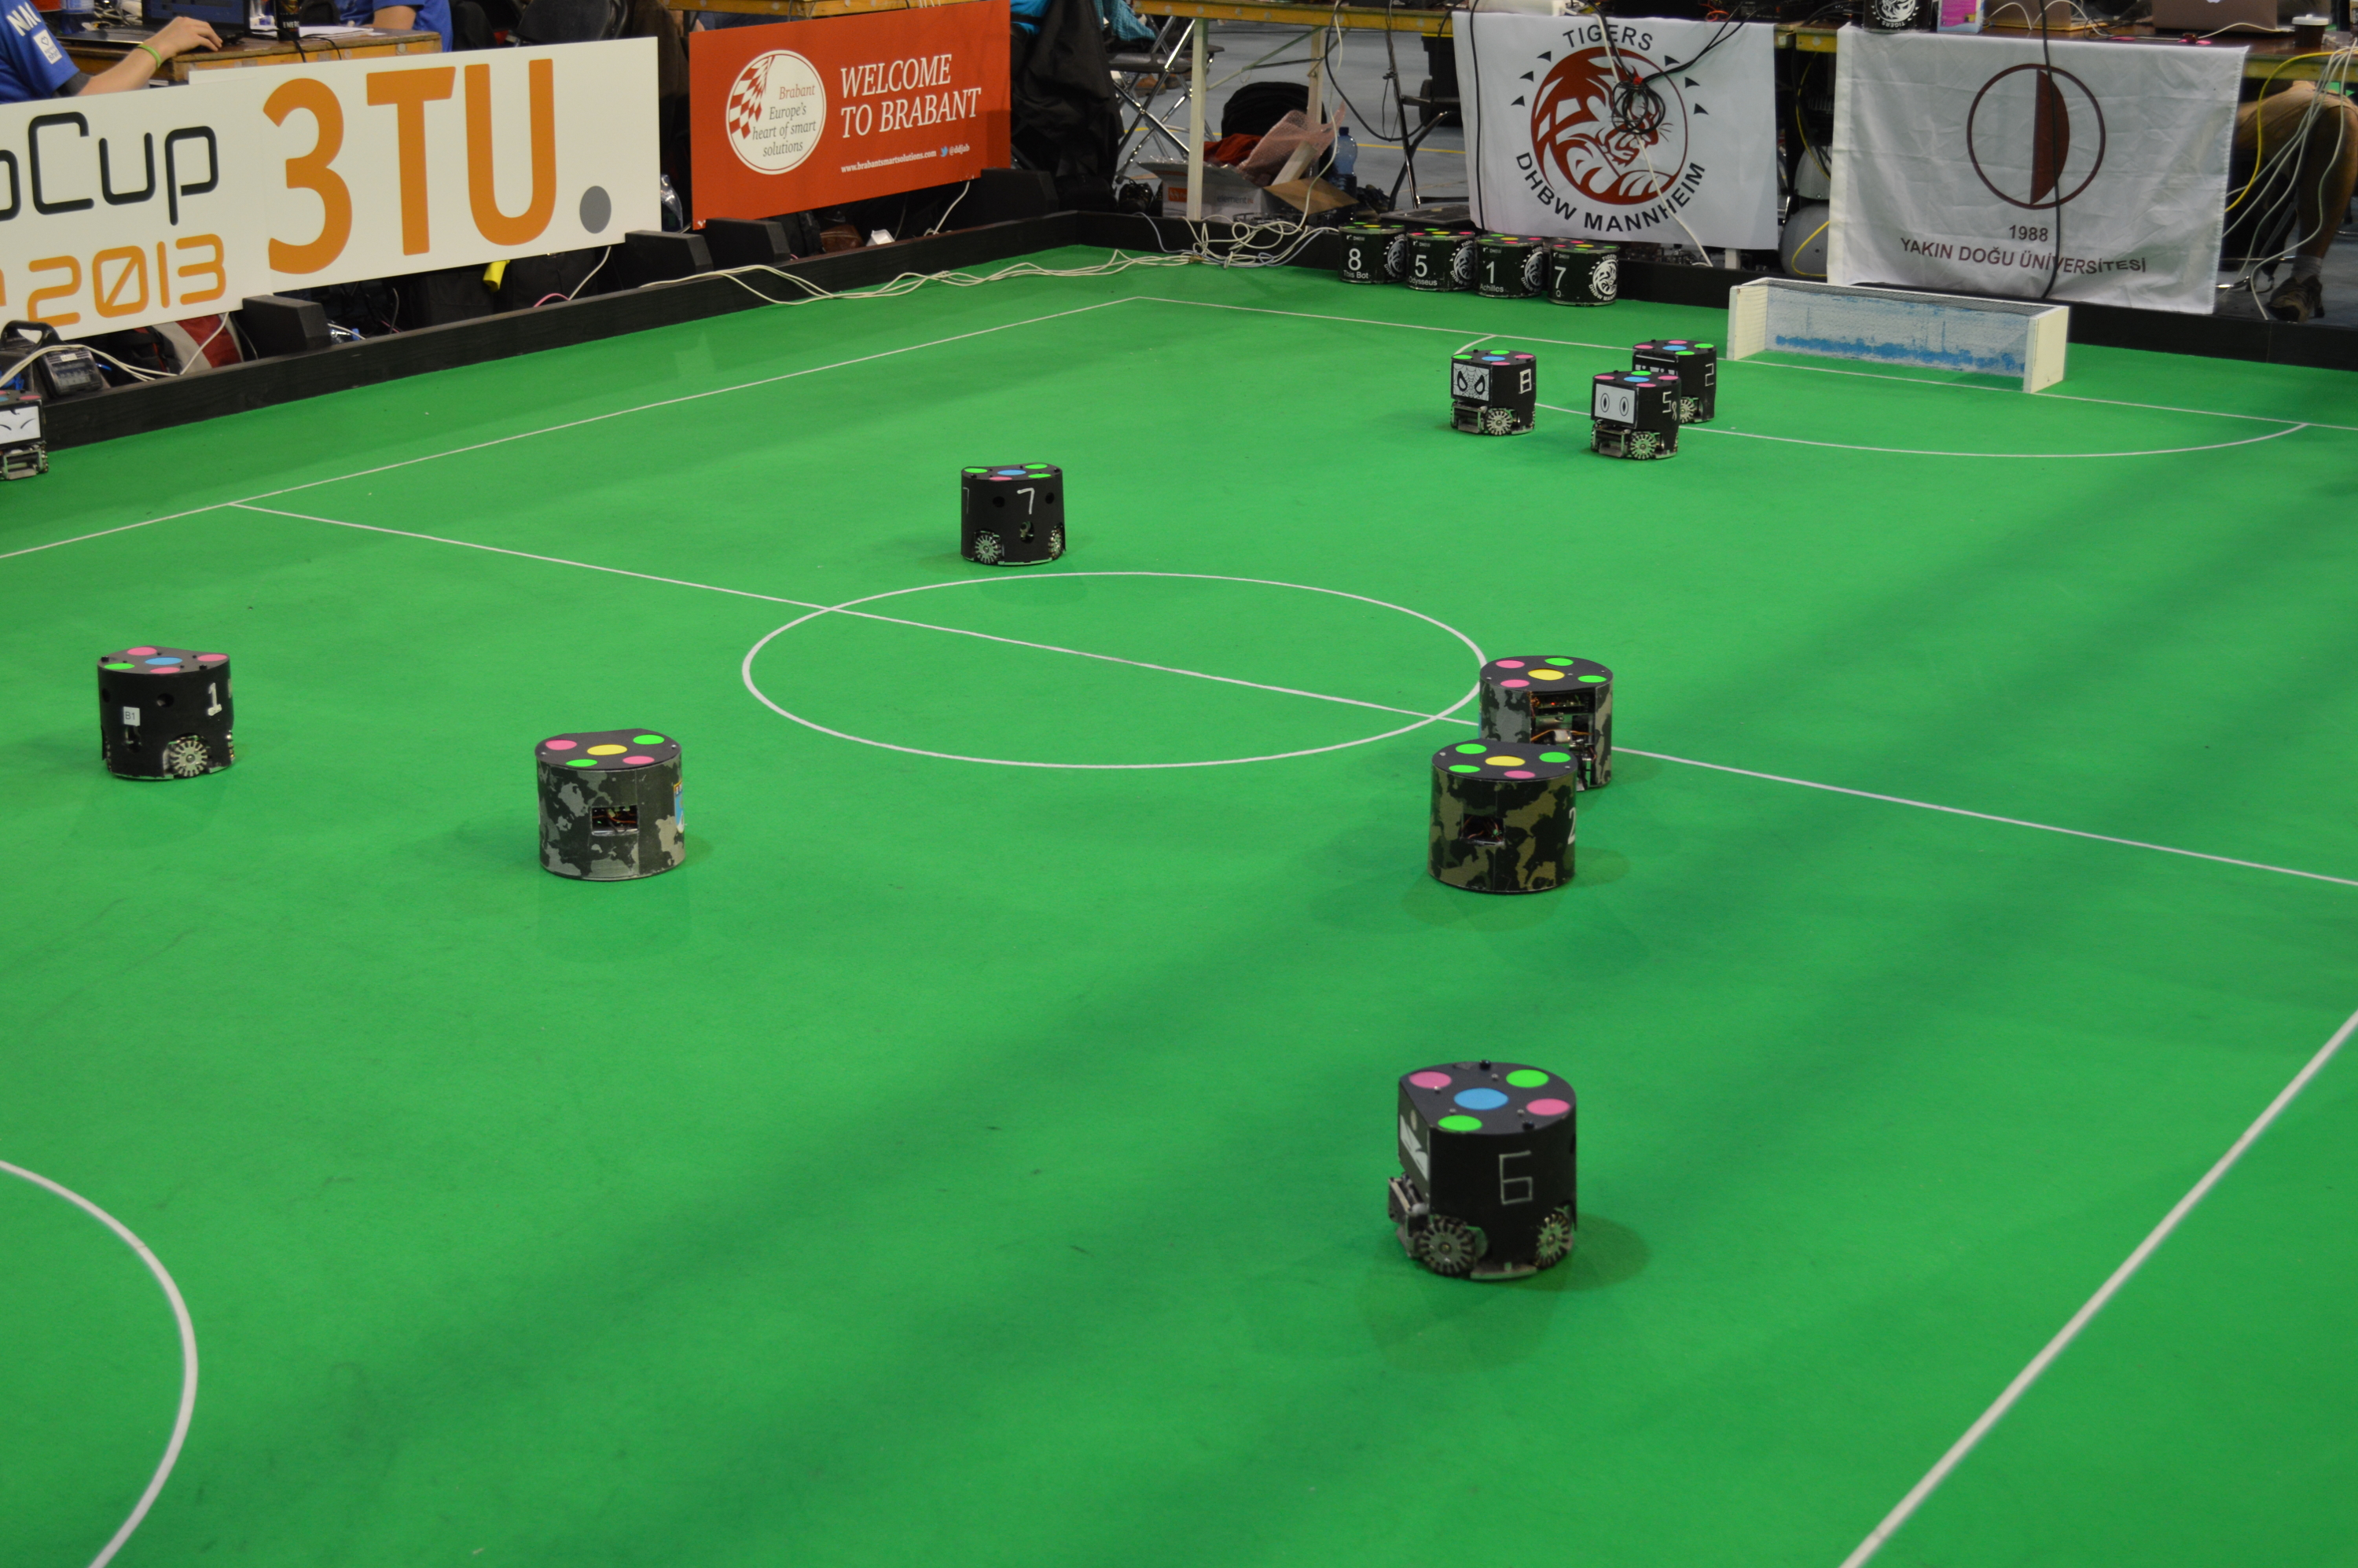
\includegraphics[width = \linewidth]{figuras/robocup2013}
  \caption{Imagem da SSL \textit{RoboCup} 2013 em Eindhoven, na Holanda}\label{fig:robocup2013}
\end{figure}

A ideia de robôs jogando futebol foi mencionada pela primeira vez pelo professor
Alan Mackworth (\textit{University of British Columbia}, Canadá) em um artigo intitulado
\textit{"On Seeing Robots"}, apresentado no \textit{Vision Interface 92} e posteriormente publicado em
um livro chamado \textit{Computer Vision: System, Theory and Applications}. Independentemente,
um grupo de pesquisadores japoneses organizou um \textit{Workshop} no \textit{Ground Challange
in Artificial Inteligence}, em Outubro de 1992, Tóquio, discutindo e propondo problemas que
representavam grandes desafios. Esse \textit{Workshop} os levou a sérias discussões sobre
usar um jogo de futebol para promover ciência e tecnologia. Estudos foram feitos para
analisar a viabilidade dessa ideia. Os resultados desses estudos mostram que
a ideia era viável, desejável e englobava diversas aplicações práticas. Em 1993, um
grupo de pesquisadores, incluindo Minoru Asada, Yasuo Kuniyoshi e Hiroaki Kitano,
lançaram uma competição de robótica chamada de Robot \textit{J-League} (fazendo uma analogia à
\textit{J-League}, nome da Liga Japonesa de Futebol Profissional). Em um mês, vários
pesquisadores já se pronunciavam dizendo que a iniciativa deveria ser estendida ao
âmbito internacional. Surgia então, a \textit{Robot World Cup Initiative} (RoboCup).

RoboCup é uma competição destinada a desenvolver os estudos na área de robótica e
Inteligência Artificial (IA) por meio de uma competição amigável. Além disso, ela tem
como objetivo, até 2050, desenvolver uma equipe de robôs humanoides totalmente
autônomos capazes de derrotar a equipe campeã mundial de futebol humano. A competição
possui várias modalidades. Neste trabalho, será analisada a \textit{Small Size Robot League} (SSL),
também conhecida como F180. De acordo com as regras da SSL, as equipes devem ser
compostas por 6 robôs, sendo um deles o goleiro, que deve ser
designado antes do início do jogo. Durante o jogo, nenhuma interferência humana é
permitida com o sistema de controle dos robôs. É fornecido aos times um sistema de
visão global e esses controlam seus robôs com máquinas próprias. O sistema de controle
dos robôs geralmente é externo e recebe os dados de um conjunto de duas câmeras
localizadas acima do campo. Esse sistema de controle processa os dados, determina qual comando deve ser executado por
cada robô e envia este comando através de ondas de rádio aos robôs. Embora seja
permitido que as equipes utilizem sistemas próprios de visão, a maioria das
<<<<<<< HEAD
equipes utiliza a visão centralizada. A figura~\ref{fig:robocup2013} mostra uma
imagem da SSL Robocup 2013, da qual o a ROBOIME (Equipe de Futebol de Robôs do
=======
equipes utiliza a visão centralizada. A figura~\ref{robocup2013} mostra uma
imagem da SSL Robocup 2013, da qual a RoboIME (Equipe de Futebol de Robôs do
>>>>>>> 2bbffc8258d22096146654d1423c9b3d9363efdb
Laboratório de Robótica do IME) participou.

\section{Motivação}

O futebol de robôs, problema padrão de investigação internacional, reúne grande parte
dos desafios presentes em problemas do mundo real a serem resolvidos em tempo real.
As soluções encontradas para o futebol de robôs podem ser estendidas, possibilitando
o uso da robótica em locais de difícil acesso para humanos, ambientes insalubres e
situações de risco de vida iminente.

Há diversas novas áreas de aplicação da robótica, tais como exploração espacial e submarina,
navegação em ambientes inóspitos e perigosos, serviço de assistência médica
e cirúrgica, além do setor de entretenimento. Essas áreas podem ser beneficiadas com o
desenvolvimento de sistemas
multi robôs. Nestes domínios de aplicação, sistemas de multi robôs deparam-se sempre
com tarefas muito difíceis de serem efetuadas por um único robô. Um time de robôs pode
prover redundância e contribuir cooperativamente para resolver o problema em questão.
Com efeito, eles podem resolver o problema de maneira mais confiável, mais rápida e
mais econômica, quando comparado com o desempenho de um único robô.

% TODO Incluir imagem do robô
%\begin{figure}
%  \includegraphics[width = \pagewidth]{}
%\end{figure}

Devido à grande complexidade do problema de interação com humanos, faz-se necessário
que os robôs sejam dotados de uma capacidade de aprendizado para facilitar a interação
desses com o mundo real. Isso é relevante tanto para aplicações industriais, quanto para
aplicações em resgates e militares. Isso diminui a necessidade de modelagem
exata dos ambientes em que os sistemas robóticos serão introduzidos e permite que
a adaptação a ambientes complexos seja realizada através da exposição destes sistemas
às possíveis situações de trabalho. Por meio da incorporação do sistema de
aprendizagem, situações não consideradas podem ser incorporadas ao algoritmo de
controle dos robôs dinamicamente. Isso permitiria que esses reagissem de maneira mais
eficiente em futuras situações semelhantes.

\section{Objetivo}

Este trabalho objetiva, através do processo de \textit{Mineração de Dados}, extrair
informação dos $logs$ (definido a seguir) de um jogo do futebol de robôs.
Isso tem o objetivo de permitir que agentes controláveis
possam reagir de maneira eficiente às ações dos agentes do time adversário, que não são controláveis.
A pesquisa se propõe a realizar esse aprendizado dos agentes adversários baseado em gravações
coletadas dos pacotes da \textit{SSL-Vision} e do \textit{Referee-Box} durante jogos, também conhecidas
como \textit{logs}, para posteriormente serem incorporados ao sistema de inteligência da
equipe de futebol de robôs do Laboratório de Robótica, denominada RoboIME.
% NOTE: acho que não é o caso disso:
%Se possível, deseja-se que essa modelagem/aprendizagem seja feita dinamicamente durante a partida da SSL.

\section{Justificativa}% TODO Maj Duarte colocou um certo nessa encestação

Um método concreto que possa prever o comportamento de agentes inteligentes de um jogo de
futebol de robôs permite com que seja possível prever o comportamento de um time adversário.
Com tal mecanismo é possível melhorar a Inteligência Artificial em uso pela RoboIME
para tomar decisões que levem a resultados melhores e, por consequência, ganhar mais partidas.
Outras equipes participantes da SSL já utilizam mecanismos de predição do adversário.
Portanto, é de grande importância desenvolver também tal mecanismo para acompanhar a evolução
das tecnologias envolvidas.

\section{Metodologia}

Para atingir os objetivos propostos, será seguida a seguinte metodologia:
Inicialmente o problema a ser investigado será definido formalmente,
utilizando definições e teorias apropriadas.

Posteriormente, a bibliografia é revisada e são evidenciados os métodos comumente
utilizados para a abordagem do problema mais geral de classificação, bem como são
analisados trabalhos aplicados especificamente à SSL.

A seguir, são analisadas as heurísticas levantadas durante a
revisão da bibliografia. Cada uma delas é descrita. Após descrição sumária
de cada heurística, são apresentados os respectivos exemplos de cada aplicação.

Então, são apresentadas abordagens envolvendo as heurísticas introduzidas
anteriormente. Cada abordagem relaciona, no mínimo, uma dessas heurísticas.
Ao final de cada seção, é apresentado uma metodologia a ser aplicada
na resolução do problema. Uma análise das características de cada abordagem
é feita ao final da descrição de cada abordagem.

<<<<<<< HEAD
A seguir, são descritos possíveis algoritmos para implementar essas abordagens.
Essas abodragens são analisadas.
=======
A seguir, são descritos possíveis algoritmos para implementar essas abordagens. Também são
desenvolvidas métricas para avaliar os algoritmos desenvolvidos.
>>>>>>> 2bbffc8258d22096146654d1423c9b3d9363efdb

% NOTE: não é bem verdade isso:
%Para validar os estudos desenvolvidos, o projeto de um software
%que analise os dados dos \textit{logs} disponíveis no site da SSL é apresentado.

\section{Estrutura do Trabalho}

No capítulo~\ref{cap:def_problema}, o problema a ser resolvido é definido formalmente.

No capítulo~\ref{cap:rev_bibliografica}, a bibliografia é revisada.

No capítulo~\ref{cap:heuristicas}, são apresentados tutoriais relacionados às
heurísticas comumente utilizadas em problemas de classificação.

No capítulo~\ref{cap:anal_abordagens}, são descritas possíveis abordagens a serem
seguidas para resolução do problema.

No capítulo~\ref{cap:conclusao}, são apresentadas as principais conclusões atingidas.

%\chapter*[Introdução]{Introdução}
%\addcontentsline{toc}{chapter}{Introdução}
%
%Este documento e seu código-fonte são exemplos de referência de uso da classe
%\textsf{abntex2} e do pacote \textsf{abntex2cite}. O documento 
%exemplifica a elaboração de trabalho acadêmico (tese, dissertação e outros do
%gênero) produzido conforme a ABNT NBR 14724:2011 \emph{Informação e documentação
%- Trabalhos acadêmicos - Apresentação}.
%
%A expressão ``Modelo Canônico'' é utilizada para indicar que \abnTeX\ não é
%modelo específico de nenhuma universidade ou instituição, mas que implementa tão
%somente os requisitos das normas da ABNT. Uma lista completa das normas
%observadas pelo \abnTeX\ é apresentada em \citeonline{abntex2classe}.
%
%Sinta-se convidado a participar do projeto \abnTeX! Acesse o site do projeto em
%\url{http://abntex2.googlecode.com/}. Também fique livre para conhecer,
%estudar, alterar e redistribuir o trabalho do \abnTeX, desde que os arquivos
%modificados tenham seus nomes alterados e que os créditos sejam dados aos
%autores originais, nos termos da ``The \LaTeX\ Project Public
%License''\footnote{\url{http://www.latex-project.org/lppl.txt}}.
%
%Encorajamos que sejam realizadas customizações específicas deste exemplo para
%universidades e outras instituições --- como capas, folha de aprovação, etc.
%Porém, recomendamos que ao invés de se alterar diretamente os arquivos do
%\abnTeX, distribua-se arquivos com as respectivas customizações.
%Isso permite que futuras versões do \abnTeX~não se tornem automaticamente
%incompatíveis com as customizações promovidas. Consulte
%\citeonline{abntex2-wiki-como-customizar} par mais informações.
%
%Este documento deve ser utilizado como complemento dos manuais do \abnTeX\ 
%\cite{abntex2classe,abntex2cite,abntex2cite-alf} e da classe \textsf{memoir}
%\cite{memoir}. 
%
%Esperamos, sinceramente, que o \abnTeX\ aprimore a qualidade do trabalho que
%você produzirá, de modo que o principal esforço seja concentrado no principal:
%na contribuição científica.
%
%Equipe \abnTeX 
%
%Lauro César Araujo


% Desenvolvimento
% ---------------

\chapter{Heurísticas para Solução do Problema}\label{cap:heuristicas}

\section{Introdução}

Esta secção tem o objetivo de apresentar um estudo dos seguintes algoritmos:
ACO, SA, ANN e GA\@. Também contém uma descrição da lógica fuzzy, inicialmente
proposta para resolver o problema.

%Várias estruturas são utilizadas em problemas de classificação. Dentre elas:

%\textit{Hidden Markov Models} (HMMs), \textit{Conditional Random Fields} (CRFs),
%Redes Neurais Artificiais (RNAs), \textit{Support Vector Machines}.

%As modelagens estudadas nesse trabalho envolvem as RNAs e CRFs.

\frame{
  \frametitle{Lógica Nebulosa}
  \begin{block}{}
    \begin{figure}
      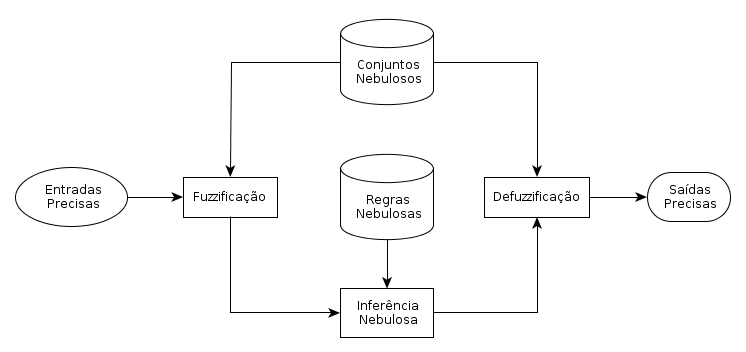
\includegraphics[width=0.8 \linewidth]
      {imgs/arquitetura_fuzzy}
      \caption{Arquitetura Funcional Genérica de um Sistema
      Nebuloso}
    \end{figure}
  \end{block}
}

\frame{
  \frametitle{Lógica Nebulosa}
  \begin{block}{}
    \textbf{Exemplo} Determinar o valor da apólice de seguro
    a ser paga pelo cliente João, cuja idade é 35 anos e a
    pressão arterial é de (130,75). As regras são:
    \begin{itemize}
      \item \emph{SE} idade é \textit{meia-idade} \emph{E}
            pressão arterial é \textit{baixa} \emph{ENTÃO}
            seguro é \textit{baixo}
      \item \emph{SE} é \textit{jovem} \emph{E} pressão
            arterial é \textit{alta} \emph{ENTÃO} seguro
            é \textit{alto}
    \end{itemize}
  \end{block}
}

%\frame{
%  \frametitle{Lógica Nebulosa}
%  \begin{block}{}
%    Se $\mu_{meia-idade}(35)= 0.8, \mu_{jovem}(35)= 0.6,
%    \mu_{Alta}(130,70)=0.5$ e $\mu_{Baixa}=0.6$, tem-se:
%    \begin{itemize}
%      \item $0.8$ \emph{E} $0.6$ = $Min \lbrace 0.8,
%      0.6\rbrace = 0.6 = \mu_{seguro-baixo}(X_1)$
%      \item $0.6$ \emph{E} $0.5$ = $Min \lbrace 0.6,
%      0.5\rbrace = 0.5 = \mu_{seguro-alto}(X_2)$
%    \end{itemize}
%  \end{block}
%  \begin{block}{}
%    Aplicando o processo de defuzzificação, obtem-se:
%    \begin{itemize}
%      \item $X_1 = 700$ e $X_2 = 800$
%    \end{itemize}
%	Assim, o valor final da apólice de seguro seria:
%	\[
%	Seguro = \frac{(0.6 \times 700)+(0.5 \times 800)}
%	{0.6+0.5} = 745.45 reais
%	\]
%  \end{block}
%}

\frame{
  \frametitle{Lógica Nebulosa}
  \begin{block}{}
    \begin{figure}
      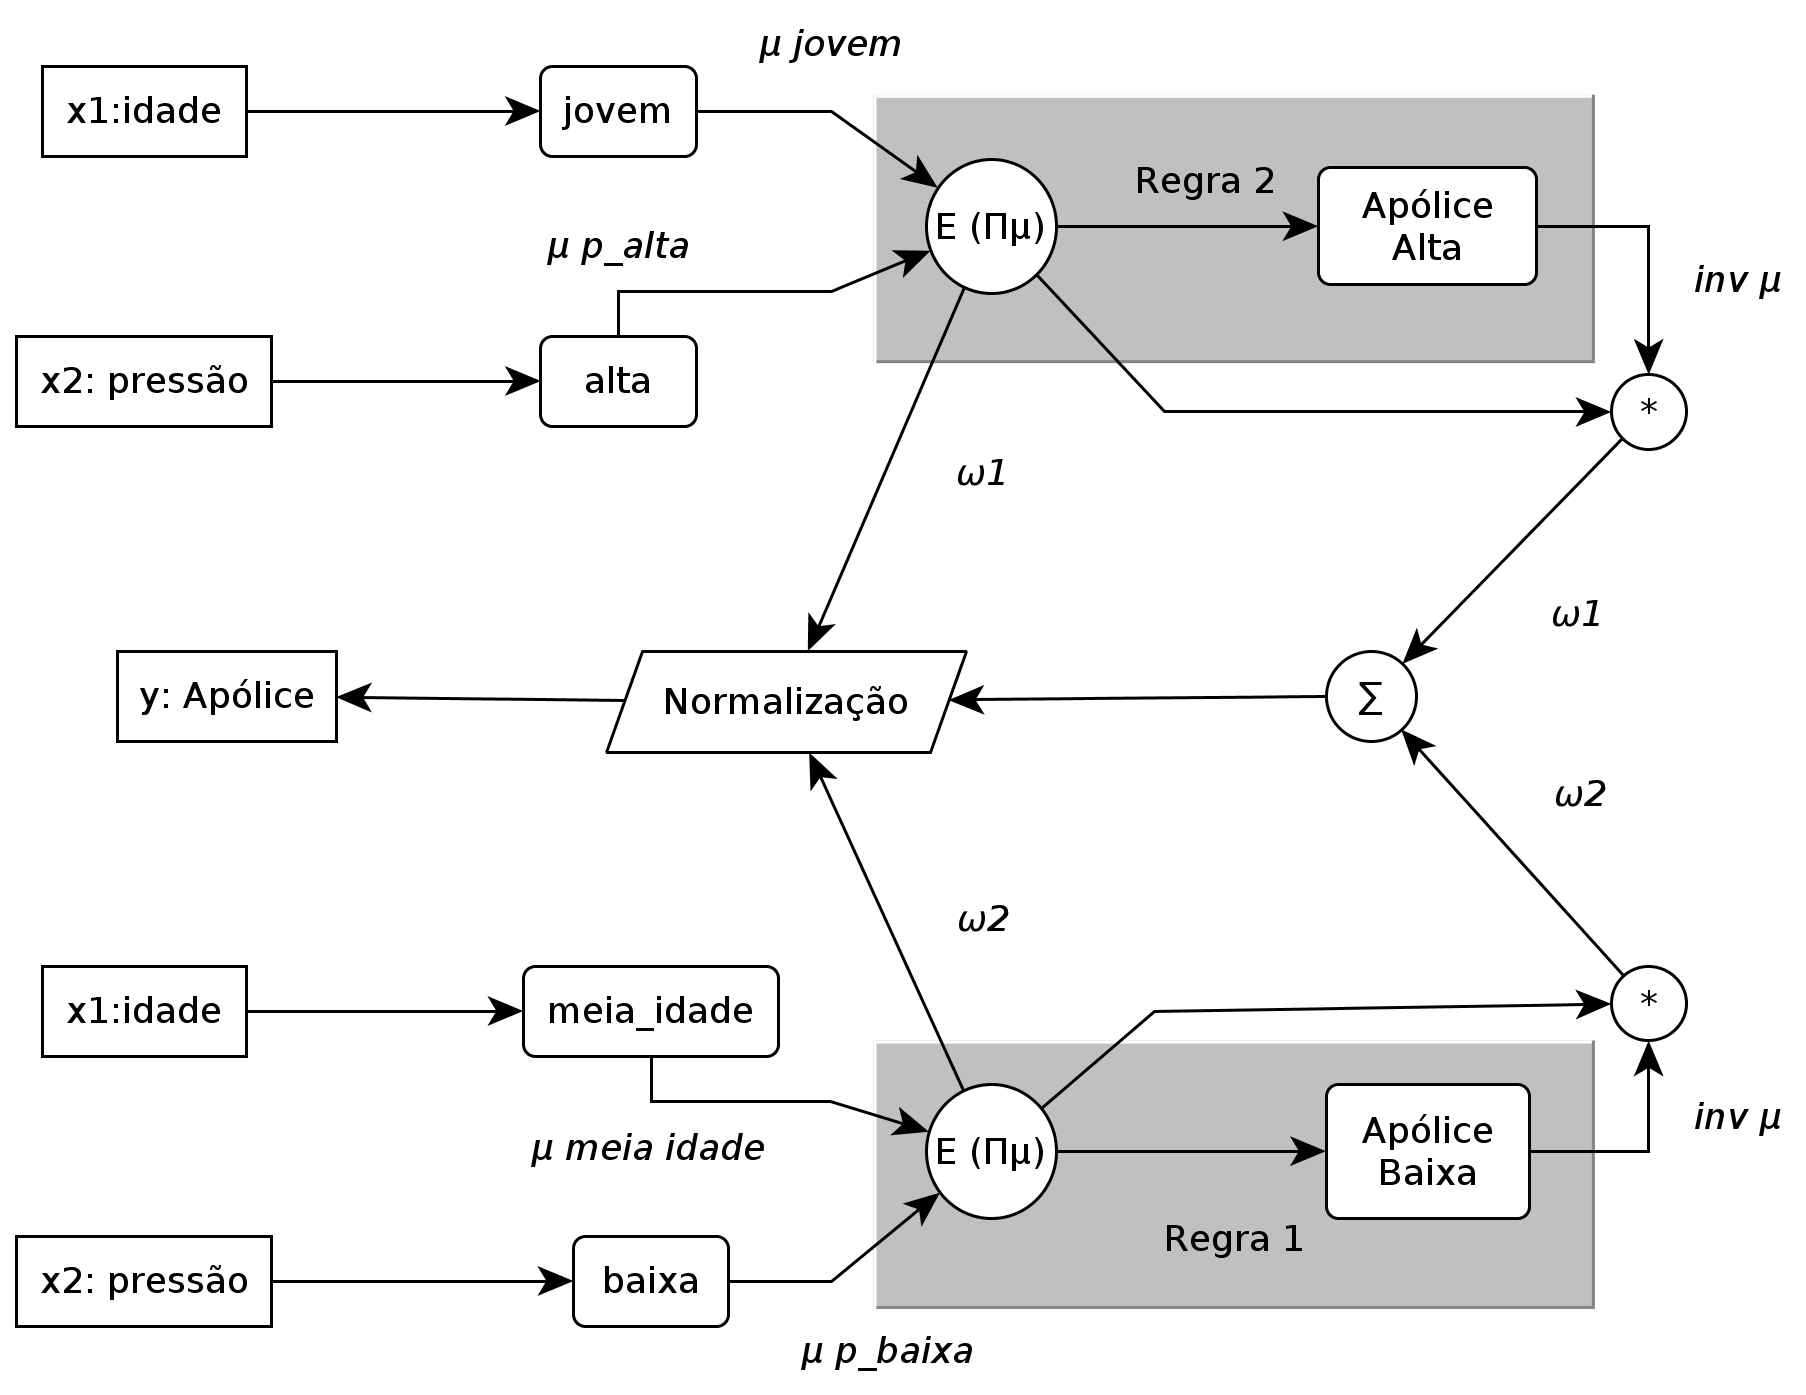
\includegraphics[width =0.6 \linewidth]
      {imgs/ex_logica_fuzzy}
      \caption{Exemplo de Aplicação}
    \end{figure}
  \end{block}
}

\frame{
  \frametitle{Lógica Nebulosa (SAM)}
  \begin{block}{}
    $$
    F(x) = \frac{\sum w_i.a_i(x).V_i.c_i}{\sum w_j.a_j(x).V_j}
    $$

    Com o volume/área $V_j$ e o centroide $c_j$ são dados por:

    $$
    V_j = \int{b_j(y_1, \cdots ,y_p)}_{\Re^{p}}.dy_1
    \cdots dy_p > 0
    $$

    $$
    c_j = \frac{\int{y.b_j(y_1,\cdots,y_p)}_{\Re^{p}}
    .dy_1 \cdots dy_p}{V_j}
    $$
  \end{block}
}

\section{Otimização da Colônia de Formigas}

Na busca por alimento, as formigas utilizam de feromônios para encontrar o melhor caminho.
Isso acontece da seguinte maneira: cada formiga deposita feromônio ao se deslocar. A partir
da avaliação da quantidade de feromônio depositada por formigas que já passaram pelo local,
formigas subsequentes tem mais probabilidade de se mover em rotas que tem mais feromônios. Ao
decorrer do tempo os feromônios vão evaporando, apagando rastros que não foram reforçados. 
Com isso, caminhos que são percorridos por mais formigas tem mais chance de serem 
percorridos por outras formigas do que aqueles que foram percorridos por menos formigas e 
caminhos que foram percorridos há pouco tempo tem mais chance de serem percorridos que caminhos
percorridos a muito tempo. A quantidade de feromônio depositado é mais intensa no trajeto de volta,
quando a comida foi encontrada. Outro fator que é levado em consideração é a qualidade da comida
encontrada, de maneira que mais feromônio é depositado quanto melhor for a fonte de alimento encontrada.
A medida que mais formigas exploram o local e encontram alimento, esse procedimento tende a otimizar o
trajeto entre a fonte de alimento e a colônia.

Apesar dessa heurística utilizada pelas formigas ser interessante para se resolver problemas combinatórios 
do tipo NP (i.e., com complexidade não polinomial), são necessárias algumas adaptações na construção
de um algoritmo computacional.

A seguir é apresentado a meta-heurística do algoritmo ACO (\textit{Ant Colony Optimization}),
juntamente com observações relacionadas as diferenças entre a heurística do ACO e o
comportamento natural das formigas descrito anteriormente.

\subsection{Meta-heurística do ACO}

\begin{figure}[ht]
  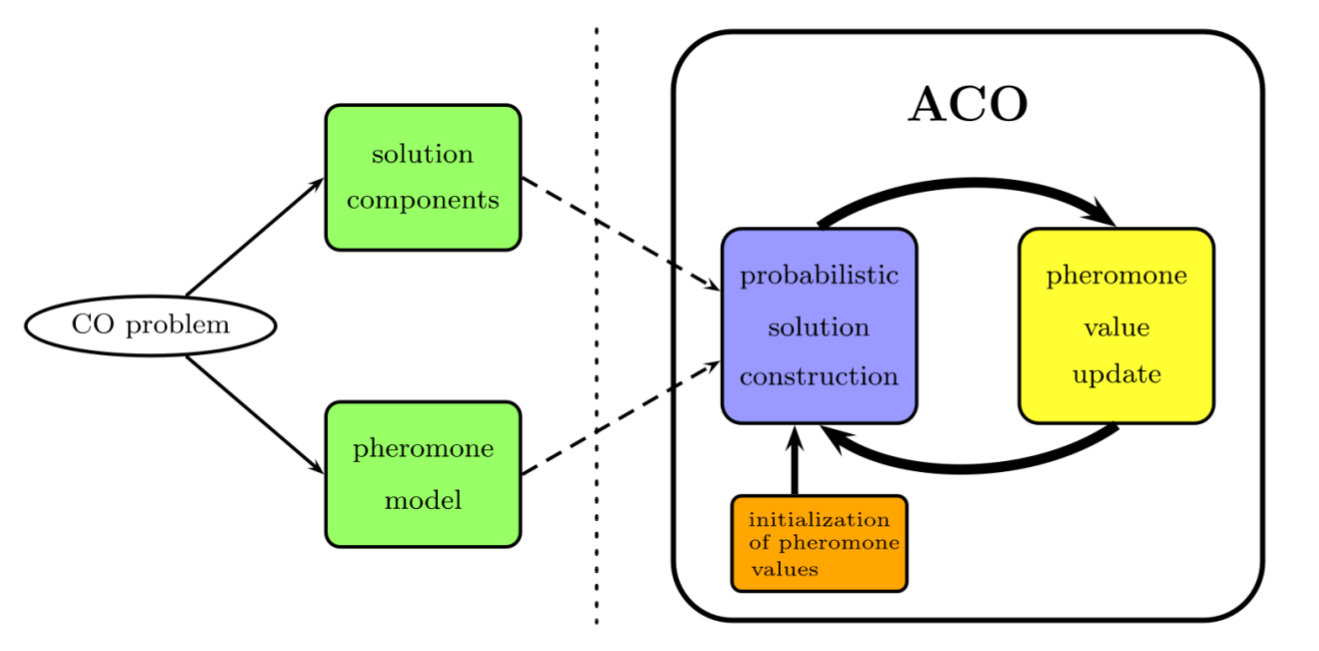
\includegraphics[width = 0.9 \linewidth]{imgs/meta_heuristica_aco}
  \caption{Diagrama de funcionamento da meta-heurística do ACO \cite{blum2005aco}}
  \label{diagrama_metaheuristica_aco}
\end{figure}

%Algoritmo
\begin{algorithm}[H]
  %Macros
  \SetKwBlock{AgendarAtividade}{AgendarAtividade}{fim}
  \SetKwBlock{Procedimento}{Procedimento}{fim}

  \Procedimento{
    \Enqto{$n < N_{MAX\_IT}$}{
      %\tcp*[f]{$N_{MAX\_IT}$ é o número máximo de iterações\\}
      \AgendarAtividade{
        ConstruirSolucoesFormigas\\
        AtualizarFeromonios\\
        %\tcp*[f]{opcional}\\
        \tcp{opcional:}
        AcoesGlobais
      }
    }
  }

  \caption{Pseudo código da meta-heurística do ACO\label{lst:meta-heuristica_aco}}
\end{algorithm}

A meta-heurística do ACO pode ser subdividida em três partes,
conforme proposto por \cite{doringo2004ant}: \textit{ConstruirSolucoesFormigas},
\textit{AtualizarFeromonios} e \textit{AcoesGlobais}.

\textit{ConstruirSolucoesFormigas} gerencia a movimentação de uma colônia de formigas
em torno dos nós vizinhos. A escolha do próximo nó é feita através de uma decisão
estocástica que é função da quantidade de feromônio no nós vizinhos e informação heurística.
Quando uma formiga encontra uma solução, ou enquanto a solução é construída, esta avalia a
qualidade da solução (completa ou parcial) que será utilizada pelo procedimento
\textit{AtualizarFeromonios} para decidir a quantidade de feromônio que será depositada.
Outro procedimento relevante na construção da solução é a eliminação de possíveis ciclos, utilizado
por exemplo, no problema do caixeiro viajante.

\textit{AtualizarFeromonios} é o processo que atualiza os traços de feromônio depositados pelas
formigas no espaço de busca. Os traços de feromônio podem aumentar, caso uma formiga tenha visitado
o nó/conexão em questão, ou diminuir, devido ao processo de evaporação do feromônio. Esse procedimento faz com 
que nós/conexões que foram visitados por muitas formigas ou por uma formiga e que tenha levado em
uma solução boa aumentem a probabilidade de serem visitados por futuras formigas. Semelhantemente, reduz 
a probabilidade de que nós que não foram visitados por novas formigas por muitas iterações sejam visitados
novamente. Logo, este procedimento evita a convergência a caminhos sub ótimos, favorecendo também a exploração
de novas regiões do espaço de busca.

Por fim, o procedimento \textit{AcoesGlobais} é utilizado para centralizar ações que não podem ser executadas
pelas formigas individualmente. Um exemplo de ações desse tipo é a filtragem de soluções ou o favorecimento de
regiões por meio de informações globais.

O procedimento \textit{AgendarAtividade} não necessariamente é uma instrução sequencial. Pode-se, portanto,
implementá-lo de maneira sequencial ou paralela, síncrona ou assincronamente. O tipo de abordagem que será
utilizada depende das características do problema que se deseja resolver.

\subsection{Exemplo de Aplicação}

\begin{figure}[ht]
  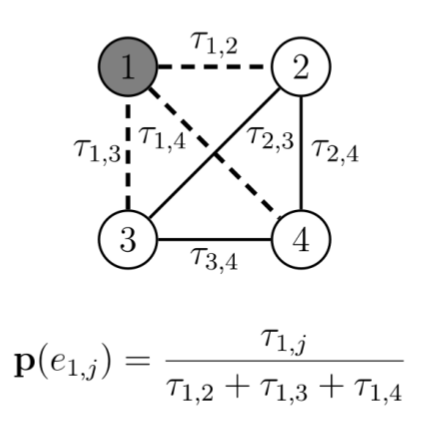
\includegraphics[width=0.32 \linewidth]{imgs/exemplo_aco_1}
  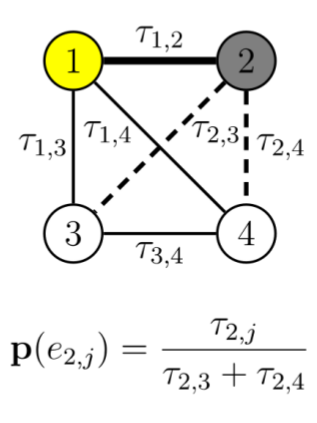
\includegraphics[width=0.32 \linewidth]{imgs/exemplo_aco_2}
  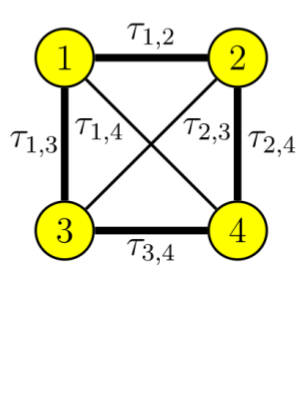
\includegraphics[width=0.32 \linewidth]{imgs/exemplo_aco_3}
  %\begin{subfigure}[b]
  %  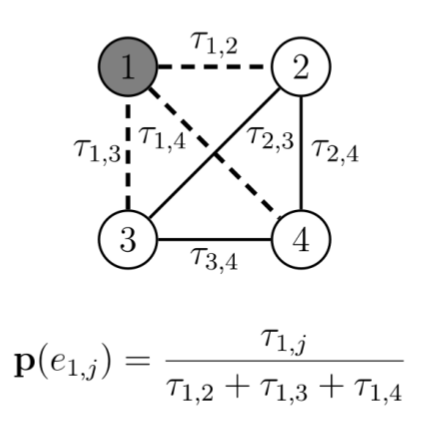
\includegraphics[width = 0.35 \linewidth]{imgs/exemplo_aco_1}
  %  \label{img:exemplo_aco_1}
  %\end{subfigure}
  %\begin{subfigure}
  %  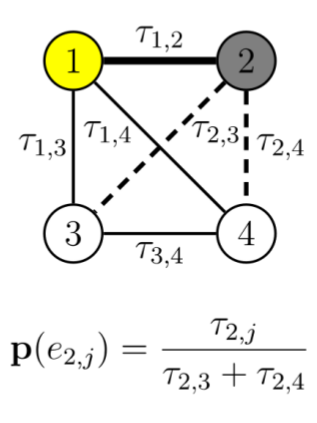
\includegraphics[width = 0.25 \linewidth]{imgs/exemplo_aco_2}
  %\end{subfigure}
  %\begin{subfigure}
  %  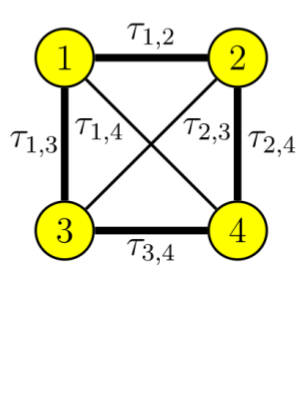
\includegraphics[width = 0.25 \linewidth]{imgs/exemplo_aco_3}
  %\end{subfigure}

  \caption{Example of the solution construction for a TSP problem}
  \label{img:exemp_aco}
  %It consists of 4 cities (modelled by a graph with 4 nodes; see Definition 1). The
  %solution construction starts by randomly choosing a start node for the ant;
  %in this case node 1. Figures (a) and (b) show the choices of the first,
  %respectively the second, construction step. Note that in both cases the
  %current node (i.e., location) of the ant is marked by dark gray color, and
  %the already visited nodes are marked by light gray color (respectively
  %yellow color, in the online version of this article). The choices of the ant
  %(i.e., the edges she may traverse) are marked by dashed lines. The probabilities
  %for the different choices (according to Eq. (4)) are given underneath the
  %graphics. Note that after the second construction step, in which we exemplary
  %assume the ant to have selected node 4, the ant can only move to node 3, and
  %then back to node 1 in order to close the tour. \cite{blum2005aco}}
\end{figure}

No TSP (\textit{Traveling Salesman Problem}) é dado um grafo completamente conectado e
não direcionado $G = (V , E)$ com pesos nas arestas.
Os nós $V$ do grafo representa as cidades e os pesos das arestas
distâncias entre as cidades. O objetivo é encontrar um caminho fechado em $G$
que contenha cada nó exatamente uma vez (portanto chamado passeio)
e cujo comprimento é mínimo. Logo, o espaço de busca $S$ consiste de todos os
passeios em $G$. O valor da função objetivo $f(s)$ de um passeio $s \in S$ 
é definido pela soma dos pesos das arestas que existem em $s$. O TSP pode ser
modelado de diversas maneiras como um problema de otimização discreta.
O modelo mais comum consiste de uma variável binária de decisão $X_e$ para
cada aresta em $G$.
Se em uma solução $X_e = 1$, então a aresta $e$ participa do passeio definido pela solução.

No que se refere abordagem do TSP usando ACO, 
as arestas de um dado grafo do TSP podem ser consideradas componentes da solução,
i.e., para cada $e_{i,j}$ é introduzido um valor de feromônio $\tau_{i,j}$. 
A tarefa de cada formiga consiste em construir uma solução plausível para o TSP, i.e.,
um passeio realizável. Em outras palavras, a noção de uma tarefa para uma formiga
muda de \textit{“escolher um caminho da colônia à fonte de comida”} para \textit{“
construir uma possível solução para o problema de otimização abordado"}. Note que com essa
mudança de tarefa, as noções de colônia e fonte de comida perdem seu significado.

Cada formiga constroem uma solução da seguinte maneira.
Primeiramente, um dos nós do grafo do TSP é aleatoriamente selecionada como sendo nó inicial.
Então, cada formiga constrói seu passeio no grafo do TSP movendo-se em cada iteração de construção
de seu nó atual (i.e., a cidade na qual ela esta localizada) á outro nó que ela ainda não visitou.
A cada passo (iteração) a aresta percorrida é adicionada a solução em construção. Quando não 
restam nenhum nó não visitado a formiga fecha o passeio movendo-se de seu nó atual até
o nó inicial, selecionado aleatoriamente no início da construção da solução. Dessa maneira a 
construção da solução implica que a formiga tem memória $T$ para armazenar os nó já
visitados. Cada iteração da solução é executado da seguinte maneira. 
Assumindo que a formiga esteja no nó $v_i$ , a subsequente iteração de solução é executada com probabilidade:

\begin{equation}
  \emph{p}(e_{i,j}) = \frac{\tau_{i,j}}{\sum_{k \in \lbrace 1,\dots,
  \vert V \vert\rbrace, v_k \not\in T}\tau_{i,k}},
  \forall j \in \lbrace 1,\dots,\vert V \vert\rbrace, v_j \not\in T
\end{equation}

Para um exemplo de tal construção de solução  veja Fig.~\ref{img:exemp_aco}.
Uma vez que todas as formigas de colônia tenham completado a construção de sua
solução, a evaporação do feromônio é executada da seguinte maneira:

\begin{equation}
  \tau_{i,j} \leftarrow (1-\rho)\cdot \tau_{i,j}, \forall \tau_{i,j}\in \mathcal{T}
\end{equation}

Onde $\mathcal{T }$ é o conjunto de todos os valores de feromônio.
Então as formigas executam seu respectivos passeios. Dessa maneira,
para cada $e_{i,j} \in s$ o seguinte feromônio é depositado:

\begin{equation}
  \tau_{i,j} \leftarrow \tau_{i,j} + \frac{Q}{f(s)}
\end{equation}

Onde $Q$ é uma constante positiva e $f(s)$ é o valor da função objetivo
da solução $s$. O sistema esta iterativamente aplicando $n_a$ 
formigas por iteração até que condição de parada
(e.g., o tempo limite) seja satisfeita.
Mesmo que o algoritmo descrito acima tenha provado que o comportamento das formigas
descrito anteriormente (no inicio da seção) pode ser transferido para um algoritmo 
de otimização discreta, foi em geral descoberto que ele é inferior aos algoritmos do estado da arte
para a solução do TSP\@. Portanto, ao longo dos anos várias extensões e aprimoramentos do algoritmo
original de resolução do TSP usando ACO foram introduzidas. Todos eles cobrem a definição de
meta-heurística do ACO,
descrito anteriormente.

\section{Recozimento Simulado}

No processo de recozimento de um metal, a quantidade de energia interna livre esta intrinsecamente
relacionada ao processo de resfriamento em que o metal é submetido. Quanto mais rápido se
resfriam um metal mais energia é armazenada internamente. Isso pode ser explicado considerando que
o tempo que a estrutura leva para atingir o estado de menor energia é maior que o disponível devido
a redução da mobilidade dos átomos com o decaimento da temperatura. Com efeito, quanto maior a taxa de
resfriamento maior o número de defeitos na estrutura do sólido e menor o tamanho médio dos grãos.
Quando se reduz a taxa de resfriamento, há uma maior chance de se atingir configurações mais estáveis.
Como resultado, a energia interna é reduzida. De acordo com \cite{bertsimas1993simulated},
pode-se modelar a probabilidade $p_{ij}$ de uma configuração atômica $\{r_i\}$ com energia $E\{r_i\}$
passar para a configuração $\{r_j\}$ com energia $E\{r_j\}$ na temperatura $T$ como:

\begin{equation}
\mbox{$p_{ij}$}=\left\{
	\begin{array}{rl}
	1 & \mbox{se $E\{r_j\} \le E\{r_i\}$} \\
	exp\left\{-\frac{(E\{r_j\}-E\{r_i\})}{k_B.T}\right\} & \mbox{se $E\{r_j\} > E\{r_i\}$}
\end{array} \right.
\end{equation}

Onde $k_B$ é a constante de Boltzmann. Para se reduzir a energia livre, é necessário que uma
rotina de resfriamento seja escolhida de acordo com o tipo de material a ser resfriado.

Conforme proposto por Kirikpartrick, Gellett e Vechin (1983) e Cerny (1985), pode-se desenvolver
uma heurística probabilística para se encontrar o mínimo global de uma função custo que possua
vários mínimos locais fazendo-se uma analogia com o fenômeno físico descrito acima. A meta-heurística
induzida por este processo é chamada de meta-heurística \textit{Simulated Annealing}(Recozimento
Simulado), ou SA, apresentado a seguir.

\subsection{Meta-heurística do SA}

De acordo com \cite{bertsimas1993simulated}, os elementos básicos da meta-heurística do SA
para a resolução de um problema combinatório são:

\begin{enumerate}
 \item Um conjunto finito $S$.
 \item Um função custo $J$ de imagem real definida em $S$. Seja $S^* \subset S$ o conjunto de todos os mínimos globais da
 função $J$, suposto subconjunto próprio.
 \item Para cada $i \in S$ um conjunto $S(i) \subset S - \{i\}$, chamado de conjunto das vizinhos de $i$.
 \item Para cada $i$, uma coleção de coeficientes positivos $q_{ij}$, $j \in S(i)$, tal que $\sum_{j \in S(i)} q{ij} = 1$.
 \item Uma função não crescente $T: \textbf{N} \rightarrow (0,\infty)$, chamada de rotina de resfriamento. Aqui \textbf{N}
 representa o conjunto de inteiros positivos, e $T(t)$ é chamada de \textit{temperatura} no tempo $t$.
 \item Um estado inicial $x(0) \in S$.
\end{enumerate}

Com base na definições acima, tem-se o seguinte pseudo código para a meta-heurística do SA:

%Algoritmo
\begin{algorithm}[H]
%Macros
\SetKwBlock{Procedimento}{Procedimento}{fim}
\SetKwBlock{EscolherVizinho}{EscolherVizinho}{fim}
\SetKwBlock{CalcTransicao}{CalcTransicao}{fim}

\Procedimento{
  SetarValoresInicias\;
  \Para{$n = 1$ até $N_{MAX\_IT}$ ou $J(x^*) \le TOL$ }{
    \Para{$k = 1$ até $N_{MAX\_IT}$ ou a solução convergir}{
      \EscolherVizinho{
        selecionar algum $j \in S(i)$\;
      }

      \CalcTransicao{
        $\Delta J \leftarrow J(j)-J(i)$\;
        \Se{$Delta J \le 0$}{
          $x(t+1) \leftarrow j$\;
          $x^* \leftarrow j$\;
        }
        \Senao{
          %$q_{ij} \leftarrow exp^{\left\{-\frac{\Delta J}{T(t)} \rigth\}}$\;\\
          $q_{ij} \leftarrow exp^{ -\frac{\Delta J}{T(t)} } $\;
          \lSe{$random() < q_{ij}$}{$x(t+1) \leftarrow j$}
          \lSenao{$x(t+1) \leftarrow i$}
        }
      }
    }
    AtualizarTemperetura\;
  }
}

\caption{Pseudo código da meta-heurística do SA\label{lst:meta-heuristica_sa}}
\end{algorithm}

No algorítimo~\ref{lst:meta-heuristica_sa}, o procedimento \textit{AtualizarTemperetura} executa a
rotina de resfriamento através da função $T(t)$ definida anteriormente. Já o procedimento
\textit{EscolherVisinho} escolhe aleatoriamente um dos elementos da vizinhança do vértice atual $i$.

\section{Algorítimo Genético}

Um \emph{algorítimo genético} é uma heurística de busca que procura
imitar a seleção natural que ocorre no processo evolucionário dos
organismos vivos.

Nessa heurística, uma população de soluções (também chamadas de
indivíduos ou fenótipos) para problemas de otimização é evoluída para
conseguir soluções melhores. Cada solução possui um conjunto de
propriedades (cromossomos ou genótipos) que podem ser mutados ou
alterados.

Os requerimentos são, tipicamente:

\begin{itemize}
\item
  uma representação genética da solução
\item
  uma função de aptidão para avaliação da solução
\end{itemize}

\subsection{O processo}

O processo é iniciado com uma população com propriedades geradas
aleatoriamente.

A iteração da heurística se da em 3 etapas:

\begin{itemize}
\item
  procriação: indivíduos são pareados e é aplicada a operação de
  cruzamento (\emph{crossover})
\item
  mutação: alguns indivíduos são selecionados e é aplicada a operação de
  mutação (\emph{mutation})
\item
  seleção: é usada a função de aptidão para descartar os indivíduos
  menos aptos restando as soluções que de fato trouxeram alguma melhora.
\end{itemize}

As condições mais comuns para terminação do processo são as seguintes:

\begin{itemize}
\item
  encontrada uma solução que atende os requisitos mínimos
\item
  número fixo de gerações alcançado
\item
  recursos alocados (tempo ou dinheiro) alcançados
\item
  a melhor solução alcançou um patamar estável em que mais iterações não
  produzem soluções melhores
\item
  inspeção manual
\end{itemize}

\subsection{Limitações}

As limitações mais comuns no emprego de um algorítimo genético são:

\begin{itemize}
\item
  Funções de avaliação computacionalmente caras tornam essa heurística
  ineficiente.
\item
  Não escala bem com a complexidade, isto é, quando o número de
  elementos expostos a mutação é grande o espaço de busca cresce
  exponencialmente. Por isso, na prática algorítimos genéticos são
  usados para, por exemplo, projetar uma hélice e não um motor.
\item
  A melhor solução é relativa às outras soluções, por isso o critério de
  parada não é muito claro em alguns problemas.
\item
  Em muitos problemas os algorítimos genéticos tendem a convergir para
  um ótimo local ou as vezes pontos arbitrários em vez do ótimo global.
\item
  É difícil aplicar algorítimos genéticos para conjunto de dados
  dinâmicos. Pois as soluções podem começar a convergir para um conjunto
  de dados que já não é mais válido.
\item
  Algorítimos genéticos não conseguem resolver eficientemente problemas
  em que a avaliação é binária (certo/errado), como em problemas de
  decisão. Nesse caso buscas aleatórias convergem tão rápido quanto essa
  heurística.
\item
  Para problemas mais específicos existem outras heurísticas que
  encontram a solução mais rapidamente.
\end{itemize}

\subsection{Pseudo código de um Algorítimo Genético}

%\begin{lstlisting}
\begin{algorithm}[H]
\SetKwBlock{Procedimento}{Procedimento}{fim}

%Algorithm: GA(n, \ki, \mu)
\Procedimento{
  %// Initialise generation 0:
  $k \leftarrow 0$\;
  $P_k \leftarrow $ população de n indivíduos escolhidos aleatoriamente\;
  %// EvaluatePk:
  %\Para{cada $i$ em $P_k$}
  %Compute fitness(i) for each i ∈ Pk;
  %Computar a $avaliacao(i)$ para cada $i$ em $P_k$\;
  %while fitness of fittest individual in Pk is not high enough;
  \Enqto{a $avaliacao(i)$ de cada $i$ em $P_k$ não for boa o suficiente}{
    %// Create generation k + 1:
    %// 1. Copy:
    %Select (1−χ)×n members ofPk and insert into Pk+1;
    Selecionar os $(1 - \chi) \times n$ membros com maior $avaliacao(i)$ de $P_k$ e inserir em $P_{k+1}$\;
    %// 2. Crossover:
    %Select χ×n members of Pk; pair them up; produce offspring; insert the offspring into Pk+1;
    Selecionar $\chi \times n$ membros de $P_k$, pareá-los e inserir a cria em $P_{k+1}$\;
    %// 3. Mutate:
    %Select µ×n members of Pk+1; invert a randomly-selected bit in each;
    Selecionar os $\mu \times n$ membros de $P_{k+1}$ com maior $avaliacao(i)$ e inverter um bit aleatório de cada membro\;
    %// Evaluate Pk+1:
    %Compute fitness(i) for each i ∈ Pk;
    %Computar a $avaliacao(i)$ para cada $i$ em $P_{k+1}$\;
    %// Increment:
    %k := k + 1;
    $k \leftarrow k + 1$\;
  }
%return the fittest individual from Pk;ut your code here.
  $melhor \leftarrow$ o membro $i$ em $P_k$ com maior $avaliacao(i)$\;
  \Retorna{$melhor$}
}
\end{algorithm}
%\end{lstlisting}

%\subsection{Referências}
%
%\begin{itemize}
%\item
%  \href{http://en.wikipedia.org/wiki/Genetic\_algorithm}{Genetic algorithm}
%\item
%  \href{http://www.cs.ucc.ie/~dgb/courses/tai/notes/handout12.pdf}{Genetic Algorithms - Derek Bridge}
%\end{itemize}

% TODO[jansegre]: exemplo de utilização
% TODO[jansegre]: como pode ser utilizado

\section{Rede Neural}

O termo mais apropriado é rede neural aritificial, já que apenas rede
neural pode se referir ao sistema biológico de nervos, no entando dado o
contexto desse texto e o uso consagrado do termo ``rede neural'', esse
será usado no lugar da versão mais explícita ``rede neural artificial''.

Uma rede neural é um sistema inspirado no sistema nervoso central (em
especial o cérebro) encontrado em muitos animais. A ideia básica é ter
um grafo em que cada nó abstrai um neurônio e é representado como uma
função, alguns desses nós são responsáveis pela observação e outros pela
saída e os nós de entrada alimentam os próximos nós até chegar nos nós
de saída. \cite{haykin2001redes}

\begin{figure}[H]
  \centering
  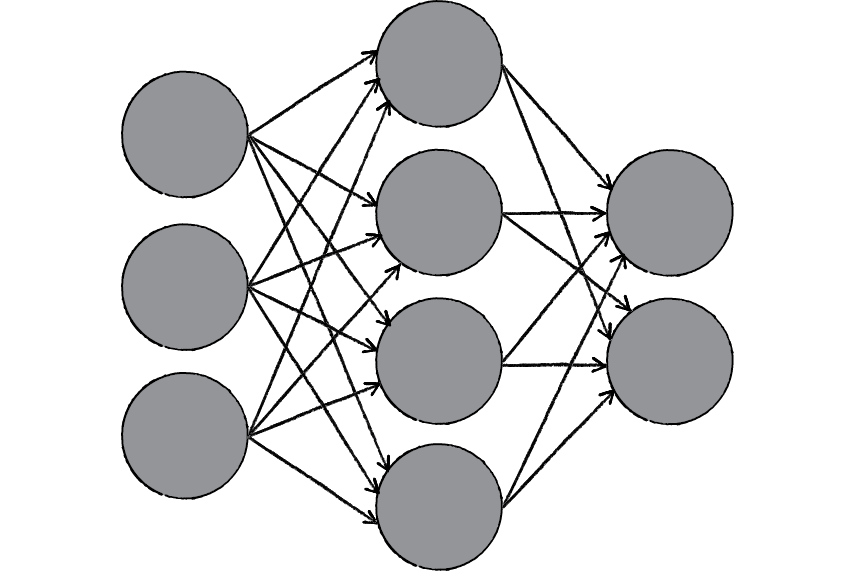
\includegraphics[width=10cm]{figuras/rede_neural_grafo}
  \caption{Rede neural com três camadas.}\label{fig:rede_neural_grafo}
\end{figure}

A figura \ref{fig:rede_neural_grafo} exemplifica uma rede neural \emph{feedforward},
que é baseada num grafo direcionado acíclico, em que podem ser vistas 3 camadas
a primeira é chamada de camada de entrada, a última, de saída e as intermediárias,
de escondidas. \cite{shiffman2012nature}

Um dos diferencias da rede neural é a capacidade de aprender, essa heurística
forma um sistem adaptativo. Existem três tipos de aprendizados:

\begin{itemize}
\item
  Aprendizado supervisionado: alimentar a rede com um problema cuja a solução é conhecida
  e depois fornecer a resposta certa para que a rede possa se ajustar.
\item
  Aprendizado não supervisionado: consiste em buscar padrões não conhecidos, não se conhece
  a resposta certa ou se uma resposta é certa ou não.
\item
  Aprendizado por reforço: alimentar a rede com um problema cuja a solução pode ser avaliada
  em boa ou má. Esse tipo de aprendizado é comum em robótica onde o robô caminha por um ambiente
  e tem o reforço negativo ou positivo de colodir ou encontrar o objetivo.
\end{itemize}

\subsection{O Neurônio}

O bloco de construção básico de uma rede neural são os neurônios.

\begin{figure}[H]
  \centering
  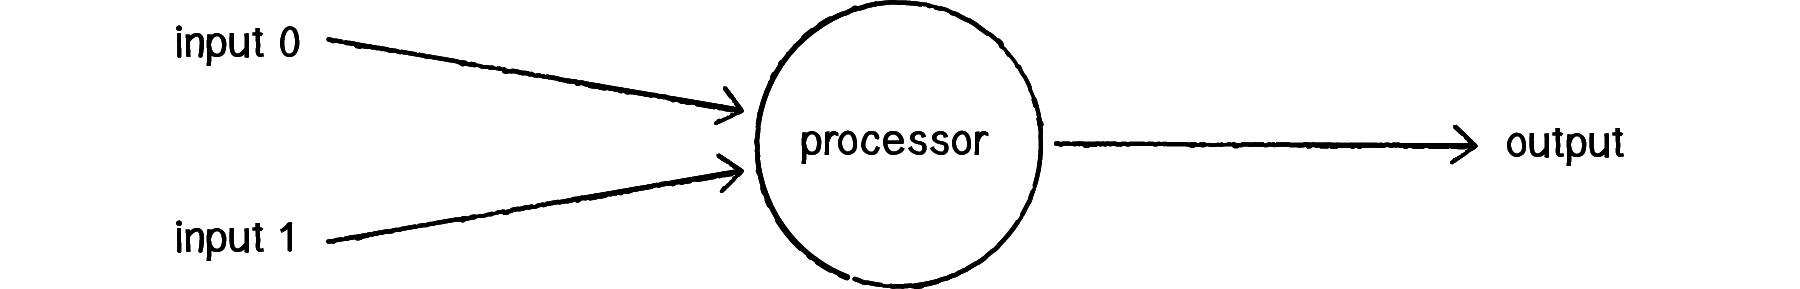
\includegraphics[width=10cm]{figuras/rede_neural_perceptron}
  \caption{Perceptron de duas entradas e uma saída.}\label{fig:rede_neural_perceptron}
\end{figure}

A figura~\ref{fig:rede_neural_perceptron} mostra um perceptron.

%\ldots{}

%\begin{itemize}
%\itemsep1pt\parskip0pt\parsep0pt
%\item
%  http://en.wikipedia.org/wiki/Neural\_network
%\item
%  http://en.wikipedia.org/wiki/Artificial\_neural\_network
%\item
%  HAYKIN, S. Redes neurais princípios e prática.
%\end{itemize}


\chapter{Análise das Possíveis Abordagens}\label{cap:anal_abordagens}

% TODO(depois): está muito obscuro, ligar com o final de cada heurística, não deve mudar muito esse capítulo.

\section{CRF}

Como os métodos AG (Algoritmo Genético), SA e ACO são heurísticas de otimização,
é necessário que o problema da aproximação de uma função seja reduzido a um problema
de otimização. A abordagem que se escolheu foi utilizar os \textit{conditional random
fields} para modelar um classificador para identificar as regras, ou táticas na
abstração da STP\@. Os métodos de otimização estudados anteriormente podem ser
aplicados para encontra os pesos do CRF.

\section{Lógica Fuzzy}

O método da Lógica Fuzzy, conforme exposto anteriormente, necessita que um conjunto
de regras seja definido. Essas regras poder ser geradas a partir de uma análise mais
detalhada do problema, mas também podem ser obtidas utilizando algum algorítimo de
aprendizagem de regras. Para aplicar esse método ao problema analisado neste trabalho
é necessário definir as regras e as distribuições das variáveis.

A vantagem dos conjuntos difusos é que eles tornam o modelo mais robusto. A lógica fuzzy
tenta melhorar a classificação e os sistemas de decisão.

A principal desvantagem deste método é a modelagem necessária para encaixar os conceitos
descritos acima. Isso, pois o conceito de conjuntos nebulosos ainda estão em desenvolvimento
para o problema abordado neste trabalho. Essa modelagem não é imediata, pois o problema é de
classificação temporal. Não basta que as características do ambiente sejam associadas aos
conjuntos nebulosos de características. É necessário que regras sejam especificadas estática
ou dinamicamente. No caso estático, elas seriam incorporadas ao modelo através de especialistas.
No caso dinâmico, uma solução é utilizar um classificador para deduzir as regras.

\section{Rede Neural}\label{cap:abordagem_rede_neural}

Essa abordagem consiste em usar uma Rede Neural que tem como entrada o estado do
jogo (todas as posições, orientações, velocidades e o comando do juiz) e como
saída o estado do time adversário (todas as posições, orientações e velocidades
dos robôs do time adversário), que visa prever as ações imediatas do adversário.
Essa rede deve ser treinada para prever um time específico usando os
\textit{logs} das partidas do torneio de 2013 da \textit{RoboCup}.

\subsection{Prova de conceito}

% TODO[jansegre] observação em <posição da bola>

Para prova de conceito, com o objetivo de estudar o pré-processamento
a ANN foi desenvolvido um programa para prever a
posição da bola. Foi implementado uma Rede Neural \textit{feedforward} com uma
camada oculta cujo
número de nós foi variado entre 8 e 320. Os nós de entrada foram 4: posições $x$
e $y$, e velocidades em $x$ e $y$, como os \textit{logs} não possuem informação
de velocidade essa foi calculada usando a diferença entre dois quadros
consecutivos. São 2 nós de saída: as posições $x$ e $y$, do próximo quadro. Foi
usada ativação sigmoid simétrica. Nessa implementação o treinamento convergiu
para um erro muito alto, como pode ser visto abaixo na saída (resumida) do
treinamento com 32 nós ocultos, é usado o erro médio quadrático e a unidade de
distância é o milímetro.

% saída do treinamento
\lstinputlisting{../train.log}

Esse problema não era esperado, foi decidido que seria necessário analisar
melhor os dados de treinamento para entender os motivos do ocorrido. Para tanto
foi modificada uma ferramenta desenvolvida no laboratório, originalmente usada
para visualizar as partidas em tempo real, a fim de visualizar os \textit{logs}
das partidas. Ao inspecionar esses logs notou-se dois tipos de irregularidades
relevantes para o treinamento, mostradas na figura~\ref{fig:logs}.

%\begin{figure}[thpb]
%  \centering
%  \begin{subfigure}[b]{0.49\textwidth}
%    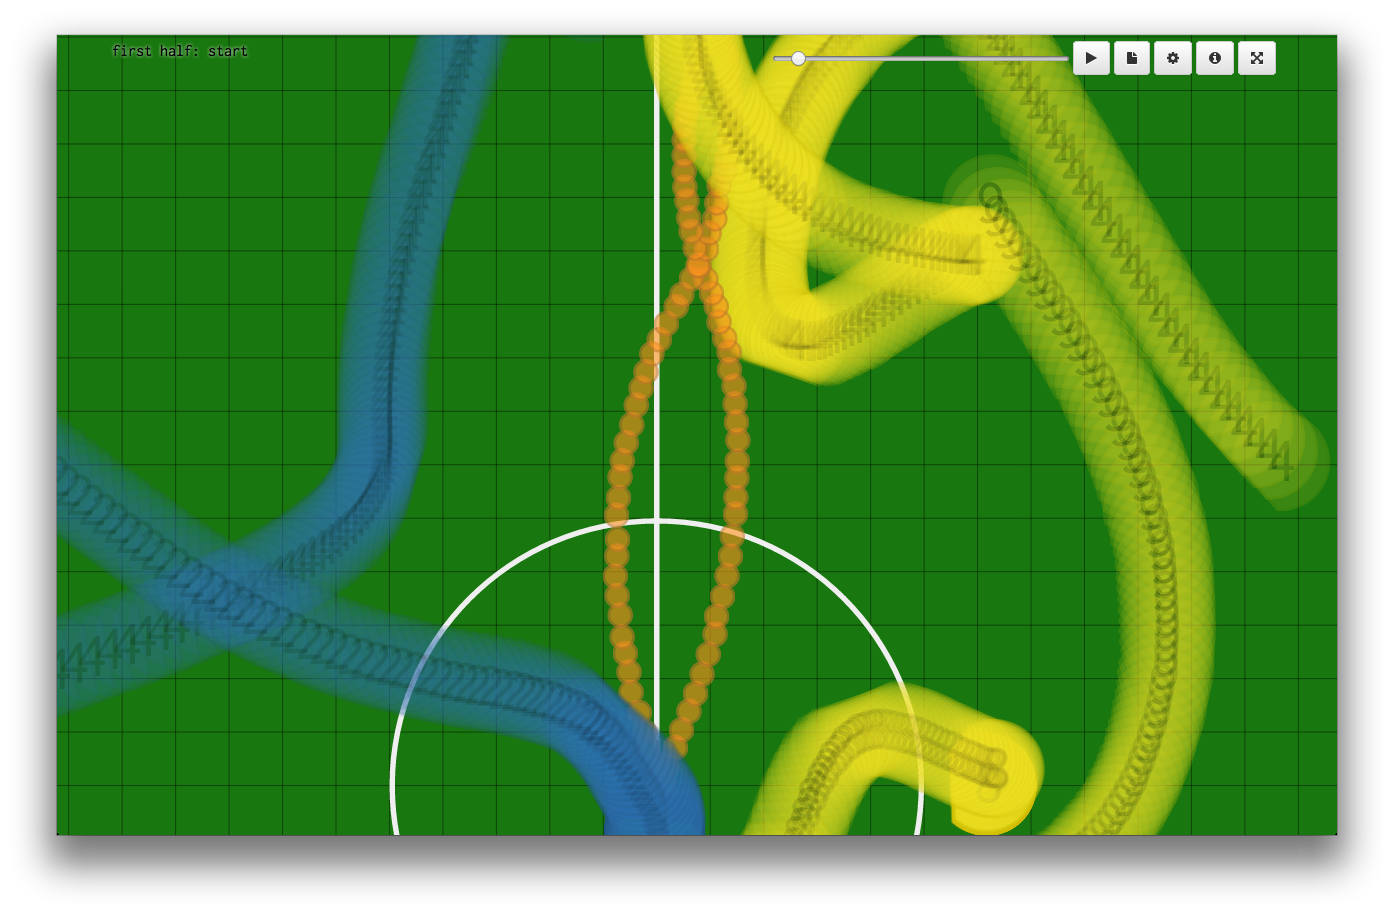
\includegraphics[width=\textwidth]{figuras/log_rastro.png}
%    \caption{Rastro duplo divergente}\label{fig:log_rastro}
%  \end{subfigure}
%  \begin{subfigure}[b]{0.49\textwidth}
%    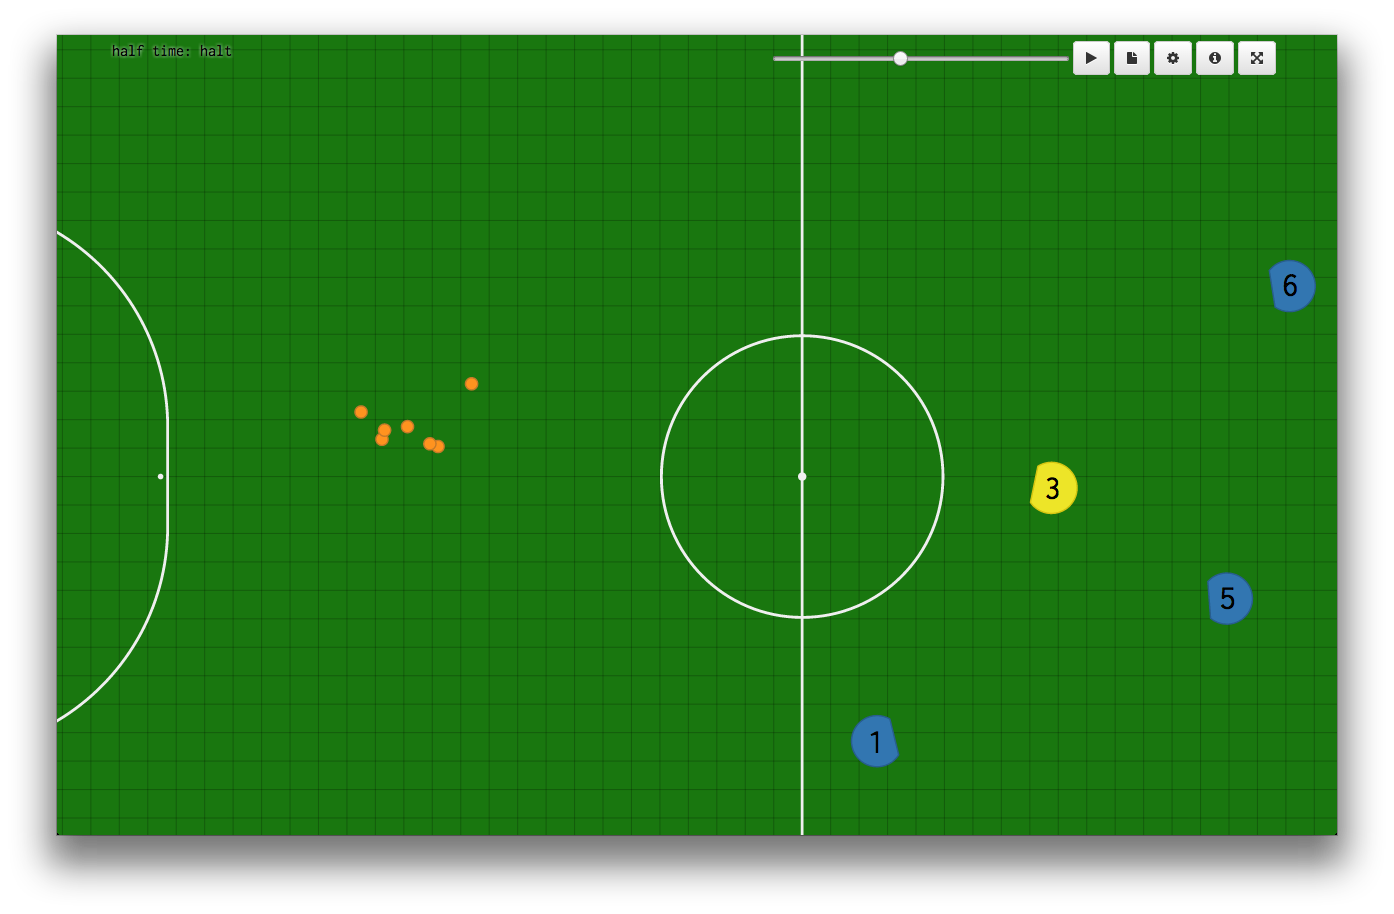
\includegraphics[width=\textwidth]{figuras/log_multi.png}
%    \caption{Objetos "fantasmas"}\label{fig:log_multi}
%  \end{subfigure}
%  \caption{Análise dos logs.}\label{fig:logs}
%\end{figure}

A figura~\ref{fig:log_rastro} mostra o problema que ocorre numa faixa no meio do
campo: a posição dos objetos (robôs e bola) oscila quadro a quadro. O motivo
desse problema é o fato das duas câmeras que capturam os dados possuírem uma
área de interseção e devido a diferenças sutis na calibração a posição dos
objetos difere quando vista de câmeras distintas. Uma saída trivial seria
ignorar os dados de uma das câmeras, mas isso é não é desejado pois uma parte
fundamental do estado do jogo estaria sendo ignorada.

Já na figura~\ref{fig:log_multi}, pode ser observado o segundo problema: há
momentos em que vários objetos "fantasmas" aparecem, isto é, são detectados
objetos que não existem no campo físico. O efeito disso é que a posição da bola
muda drasticamente para pontos que não fazem sentido.

A abordagem da rede neural, apesar de ocultar a semântica da relação dos fatores
analisados, parece bem apta a resolver o problema. Porém é necessário contornar
o problema dos dados de treinamento para poder implementar uma solução de fato.

% vim: tw=80 et ts=2 sw=2 sts=2



% modelagem é tipo uma introducao
%\section{Modelagem}

Pode-se observar que, como os métodos \textbf{Algorítmos Genéticos},
\textbf{\emph{Simulated Annealing}} e \textbf{\emph{Ant Colony
Optmization}} necessitam que um problema de otimazação seja definido.
Logo é necessário definir um modelo do problema e uma função associada
ao modelo para serem implementados. Isso implica que é necessário
definir a arquitetura da inteligência a ser modelada. Logo, para que
seja possível a modelagem de diferentes inteligências, será necessário
analizar a eficiência da otmização de cada arquitetura para que seja
escolhida a mais eficiente.

O método da Lógica Fuzzy também necessita que uma modelagem para o
sistema a ser considerado seja definida. Isso também restringe a
generalidade dos modelos que se enquadram nessa modelagem.

Já o a \textbf{Rede Neural} define implicitamente a estrutura interna
que mnimiza a diferença entre a saída real e a saída desejada.
Entretanto, é necessário definir a topologia mais adequada para o
problema em questão. Também, apezar de não ser necessário, pode-se
decompor o problema em subproblemas e ``atribuir redes neurais um
subconjunto de tarefas que coincidem com suas capacidades
inerentes''(pag. 29 HAYKIN, 2001) com o objetivo de aumentar a
adaptabilidade da rede. Apesar de ser uma modelagem para a arquitetura
da inteligência a ser mapeada, não representa uma restrição tão
consideravel quando a das abordagens citadas anteriormente.


\section{Cronograma}
\frame{
  \frametitle{Cronograma}
  \begin{block}{}
    \begin{figure}
      \centering
      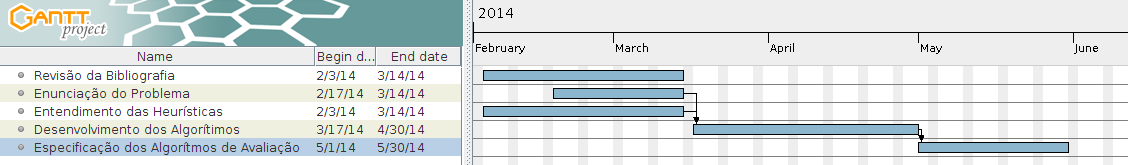
\includegraphics[width = 0.8 \linewidth]{imgs/cronograma}
      \caption{Cronograma de Atividades}
    \end{figure}
  \end{block}
}

% ----------------------------------------------------------
% PARTE - preparação da pesquisa
% ----------------------------------------------------------
%\part{Preparação da pesquisa}

% ----------------------------------------------------------
% Capitulo com exemplos de comandos inseridos de arquivo externo 
% ----------------------------------------------------------

%\include{abntex2-modelo-include-comandos}

% ----------------------------------------------------------
% Parte de revisão de literatura
% ----------------------------------------------------------
%\part{Referenciais teóricos}

% ---
% Capitulo de revisão de literatura
% ---
%\chapter{Lorem ipsum dolor sit amet}

% ---
%\section{Aliquam vestibulum fringilla lorem}
% ---

%\lipsum[1]

%\lipsum[2-3]

% ----------------------------------------------------------
% Resultados
% ----------------------------------------------------------
%\part{Resultados}

% ---
% primeiro capitulo de Resultados
% ---
%\chapter{Lectus lobortis condimentum}

% ---
%\section{Vestibulum ante ipsum primis in faucibus orci luctus et ultrices
%posuere cubilia Curae}
% ---

%\lipsum[21-22]

% ---
% segundo capitulo de Resultados
% ---
%\chapter{Nam sed tellus sit amet lectus urna ullamcorper tristique interdum
%elementum}
%
%\section{Pellentesque sit amet pede ac sem eleifend consectetuer}
%
%\lipsum[24]

% ---
% Finaliza a parte no bookmark do PDF, para que se inicie o bookmark na raiz
% ---
\bookmarksetup{startatroot}%
% ---

% ---
% Conclusão
% ---
%\chapter*[Conclusão]{Conclusão}
%\addcontentsline{toc}{chapter}{Conclusão}
\chapter{Próximas Etapas}

As próximas etapas consistem em estudar a solução através dos métodos e das abordagens 
propostas de problemas mais simples para consolidar o estudo dos métodos estudados e 
analisar as topologias das redes neurais para que futuramente seja possível encontrar 
a topologia ótima e assim refinar os resultados da rede e das regras do sistema difuso.


%\chapter{Conclusão}
% TODO(depois): Fazer uma conclusão!


%\lipsum[31-33]

% ----------------------------------------------------------
% ELEMENTOS PÓS-TEXTUAIS
% ----------------------------------------------------------
\postextual


% ----------------------------------------------------------
% Referências bibliográficas
% ----------------------------------------------------------
%\bibliographystyle{plainnat}%abbrvnat, unsrtnat, apsrev, rmpaps, IEEEtranN, achemso, rsc
\bibliography{referencias}

% ----------------------------------------------------------
% Glossário
% ----------------------------------------------------------
%
% Consulte o manual da classe abntex2 para orientações sobre o glossário.
%
%\glossary

% ----------------------------------------------------------
% Apêndices
% ----------------------------------------------------------

% ---
% Inicia os apêndices
% ---
%\begin{apendicesenv}

% Imprime uma página indicando o início dos apêndices
%\partapendices

% ----------------------------------------------------------
%\chapter{Quisque libero justo}
% ----------------------------------------------------------

%\lipsum[50]

% ----------------------------------------------------------
%\chapter{Nullam elementum urna vel imperdiet sodales elit ipsum pharetra ligula
%ac pretium ante justo a nulla curabitur tristique arcu eu metus}
% ----------------------------------------------------------
%\lipsum[55-57]

%\end{apendicesenv}
% ---


% ----------------------------------------------------------
% Anexos
% ----------------------------------------------------------

% ---
% Inicia os anexos
% ---
%\begin{anexosenv}

% Imprime uma página indicando o início dos anexos
%\partanexos

% ---
%\chapter{Morbi ultrices rutrum lorem.}
% ---
%\lipsum[30]

% ---
%\chapter{Cras non urna sed feugiat cum sociis natoque penatibus et magnis dis
%parturient montes nascetur ridiculus mus}
% ---

%\lipsum[31]

% ---
%\chapter{Fusce facilisis lacinia dui}
% ---

%\lipsum[32]

%\end{anexosenv}

%---------------------------------------------------------------------
% INDICE REMISSIVO
%---------------------------------------------------------------------

\printindex

\end{document}
